\documentclass[a4paper]{article}
\usepackage[utf8]{inputenc}
\usepackage[spanish]{babel}


\usepackage{amsmath}
\usepackage{amsfonts}
\usepackage{hyperref}
\usepackage{braket}
\usepackage{comment}

\usepackage[qm]{qcircuit}

\usepackage{graphicx}
\graphicspath{ {./imagen/} }

%\usepackage{enumerate}
%\usepackage{blindtext}

\usepackage[left=3.25cm,top=3cm,right=2cm,bottom=3.25cm]{geometry}

%Nuevos entornos
\newtheorem{deff}{Definición}[section]

%Enumeración
\numberwithin{equation}{section}

%Nuevo comandos
\newcommand\norm[1]{\lVert#1\rVert}

\title{Computación Cuántica}
\author{Chenjie Huang}
\date{}


%Documento

\begin{document}
\maketitle

\tableofcontents

\newpage

\thispagestyle{empty}

\newpage

\section{Introducción}

Alguna breve introducción y tal???

\subsection{Objetivos}

(Pendiente)

\begin{itemize}
\item Introducción a la computación cuántica. Como la metodología de trabajo. Teoría matemática, espacios de Hilbert y Producto tensorial.

\item Estructura básica, qubits, y puertas cuánticas.

\item Algoritmos cuánticos. Con ejemplos en qiskit.

\begin{itemize}
	\item Algoritmo de Deutsch
	\item Algoritmo de Deutsch-Jozsa
	\item Algoritmo de Búsqueda de Grover
	\item Algoritmo de Periodicidad de Simon
	\item Algoritmo de Factorización de Shor.
\end{itemize}

\end{itemize}

\subsection{Metodología}
Lectura parcial de los libros que ha recomendado el tutor, seguidos de su discusión e implementación en Qiskit.(?)

\section{Preliminares}

La Teoría Cuántica se apoya principalmente sobre álgebra lineal, concretamente sobre el espacio vectorial complejo de dimensión finita $\mathbb{C}^n$.
En esta sección que servirá como preliminares como indica el título, nos centraremos en la teoría de álgebra lineal sobre el espacio vectorial complejo. 

%Estudiaremos los conceptos básicos de este campo y describiremos la notación estándar utilizada en el área de estudio de la mecánica cuántica.%

El objetivo es conseguir que este apartado sirva a modo de fundamento y bases para secciones posteriores y también de consulta posteriormente.

\subsection{Espacios Vectoriales}

%Recordaremos la definición de espacio vectorial y nos familiarizaremos con la notación braket.%(???)

\begin{deff}

Un espacio vectorial sobre un cuerpo $\mathbb{K}$ es un conjunto no vacío $\mathbb{V}$, cuyo elementos llamaremos vectores, y llevan asociado dos operaciones, 
\begin{itemize}

\item La Suma, $\textbf{+}: \mathbb{V} \times \mathbb{V} \longrightarrow \mathbb{V}$

\item El Producto por un escalar, $\textbf{$\cdot$}:\mathbb{K} \times \mathbb{V} \longrightarrow \mathbb{V}$

\end{itemize}
tal que $(\mathbb{V},+)$ cumple las propiedades de formar un \textbf{grupo abeliano} y el producto por un escalar $\cdot$ cumpla las propiedades de:
\begin{itemize}

\item Existencia de elemento neutro:
\begin{equation}
\exists e \in \mathbb{K} \text{ tal que } \forall v \in \mathbb{V},  e \cdot v = v
\end{equation}

\item Propiedad asociativa:
\begin{equation}
\forall a, b \in \mathbb{K}, \forall v \in \mathbb{V}, a\cdot(b\cdot v) = (a\cdot b)\cdot v
\end{equation}

\item Propiedad distributiva respecto a la suma de vectores:
\begin{equation}
\forall a \in \mathbb{K}, \forall u, v \in \mathbb{V}, a\cdot(u + v) = a\cdot u + a\cdot v
\end{equation}

\item Propiedad distributiva respecto a la suma de escalares:
\begin{equation}
\forall a, b \in \mathbb{K}, \forall v \in \mathbb{V}, (a + b)\cdot v = a\cdot v + b\cdot v
\end{equation}

\end{itemize}

\end{deff}

En el caso de que el cuerpo de escalares sea el de los complejos $\mathbb{C}$, se le denominará \textbf{espacio vectorial complejo}, siendo estas de gran interés para nuestro campo de estudio que es la mecánica cuántica.

A partir de ahora usaremos $\mathbb{C}$ como cuerpo de escalares del espacio vectorial junto a la notación estándar de mecánica cuántica para referirnos a los elementos básicos de la álgebra lineal.

Denotaremos al vector en un espacio vectorial $\mathbb{V}$ como $\ket{v}$, donde usaremos $\ket{\cdot}$ para indicar que es un vector del espacio, denominado \textbf{\textit{ket}}.

En cuanto al elemento neutro del espacio vectorial, el vector cero, lo denotaremos excepcionalmente como $\mathbf{0}$. Veremos posteriormente que usaremos $\ket{0}$ para referirnos a algo completamente diferente.

Centrándonos más en $\mathbb{C}^n$, el espacio vectorial complejo cuyo elementos son $n$-tuplas $(z_1, z_2, \ldots z_n)$, usaremos a veces la notación de vector columna:
$$\begin{bmatrix}
z_1 \\ z_2 \\ \vdots \\ z_n
\end{bmatrix}$$

\subsection{Bases y dimensión}

\begin{deff} Sea $\ket{v_1},\ket{v_2}, \ldots, \ket{v_n}$ vectores de un cierto espacio vectorial $\mathbb{V}$ sobre $\mathbb{C}$. Diremos que un vector $\ket{v}\in\mathbb{V}$ es \textbf{combinación lineal} de ellos si existen $a_1, a_2, \ldots, a_n \in \mathbb{C}$ escalares tal que podemos escribir $\ket{v}$ como:
\begin{equation}
\ket{v} = \sum_{i=1}^n a_i \cdot \ket{v_i}
\end{equation}
\end{deff}

\begin{deff} Sea $\{ \ket{v_1},\ket{v_2}, \ldots, \ket{v_n} \}$ un conjunto de vectores de un cierto espacio vectorial $\mathbb{V}$ sobre $\mathbb{C}$. Diremos que son \textbf{linealmente dependientes} si existen $a_1, a_2, \ldots, a_n \in \mathbb{C}$, con algún $a_i \neq 0$, tal que
\begin{equation}
a_1\ket{v_1} + a_2\ket{v_2} + \ldots + a_n\ket{v_n} = 0
\end{equation}

Además diremos que son \textbf{linealmente independientes} si no son linealmente dependientes. Es decir, si existe una combinación lineal de ellos, entonces los coeficientes son todos nulos.
\end{deff}

\begin{deff} Llamaremos entonces al conjunto $B = \{ \ket{v_1},\ket{v_2}, \ldots, \ket{v_n} \}$ \textbf{base} del espacio $\mathbb{V}$ si:
\begin{itemize}
\item $B$ es linealmente independiente.

\item $\forall \ket{v} \in \mathbb{V}$, $\ket{v}$ puede ser escrito como combinación lineal de vectores de $B$.
\end{itemize}
\end{deff}

Además podemos asegurar la existencia de este conjunto para todo espacio vectorial. Y también de que el número de elementos de dos bases distintas del mismo espacio vectorial coincide y nos referiremos a este número como \textbf{dimensión} del espacio $\mathbb{V}$.

Como hemos hecho mención antes, nuestro interés se halla en espacios vectoriales de dimensión finita, por tanto haremos omiso de las cuestiones relacionadas con espacios de dimensión infinita.

\subsection{Aplicaciones lineales y forma matricial}

\begin{deff} Una aplicación lineal entre dos espacios vectoriales $\mathbb{V}$ y $\mathbb{W}$ sobre el mismo cuerpo $\mathbb{C}$ es una aplicación $f: \mathbb{V} \longrightarrow \mathbb{W}$ tal que es lineal sobre sus componentes, es decir, si $\ket{v} = \sum_{i=1}^n a_i \cdot \ket{v_i}$ entonces se cumple:
\begin{equation} \label{eq7}
f(\ket{v}) = f(\sum_{i=1}^n a_i \cdot \ket{v_i}) = \sum_{i=1}^n a_i \cdot f(\ket{v_i})
\end{equation}

Diremos además que una aplicación lineal está definida sobre $\mathbb{V}$ para referirnos a que es una aplicación lineal de $\mathbb{V}$ a $\mathbb{V}$
\end{deff}

Un aplicación de gran importancia es la aplicación identidad, que denotaremos con $id_{\mathbb{V}}$ y cumple la propiedad de que $\forall \ket{v}\in\mathbb{V}$, $id_{\mathbb{V}}(\ket{v}) = \ket{v}$.

Observando la expresión \ref{eq7} podemos llegar a la conclusión de que una aplicación lineal está completamente determinada por su acción sobre los elementos de una base, pues todo vector se puede expresar como combinación lineal de los vectores de una base.

Una manera muy útil de expresar una aplicación lineal es a través de su expresión matricial. Veamos esto con la aplicación de $f:\mathbb{V} \longrightarrow \mathbb{W}$ sobre los vectores de las bases correspondientes. Sea $\{ \ket{v_1}, \ldots, \ket{v_m} \}$ y $\{ \ket{w_1}, \ldots, \ket{w_n} \}$ bases correspondientes a $\mathbb{V}$ y $\mathbb{W}$.

Entonces para cada j de $1$ a $m$ existirán $a_{1j}, \ldots, a_{nj} \in \mathbb{C}$ tal que
\begin{equation} \label{eq8}
f(\ket{v_j}) = \sum_{i=1}^n a_{ij} \ket{w_i}
\end{equation}
por ser $f(\ket{v_j}) \in \mathbb{W}$ y $\{ \ket{w_1}, \ldots, \ket{w_n} \}$ base de $\mathbb{W}$.

\begin{deff}Llamaremos entonces $A$ a la matriz formada por los elementos $a_{ij}$ de la ecuación \ref{eq8} en la posición $(ij)$ en la matriz, como representación matricial de la función $f$.
\end{deff}

Además, tomando las \textbf{coordenadas} $\boldsymbol{z_j}$ de un vector $\ket{v} = \sum_{j=1}^m \boldsymbol{z_j} \ket{v_j}$ de $\mathbb{V}$ y su imagen por $f$ con la expresión \ref{eq8}:
\begin{equation}
f(\ket{v}) = f(\sum_{j=1}^m z_j \ket{v_j}) = \sum_{j=1}^m z_j f(\ket{v_j}) = \sum_{j=1}^m z_j (\sum_{i=1}^n a_{ij} \ket{w_i}) = 
\sum_{i=1}^n (\sum_{j=1}^m a_{ij} z_{j}) \ket{w_i}
\end{equation}
podemos observar la aplicación de $f$ sobre el vector $\ket{v}$ no es más que el producto de la matriz $A$ con el vector $\ket{v}$ en columnas:
\begin{equation}
A\ket{v} = 
\begin{bmatrix}
a_{11} & a_{12} &\ldots & a_{1m} \\
a_{21} & a_{22} &\ldots & a_{2m} \\
\vdots & \vdots &\ddots & \vdots \\
a_{n1} & a_{n2} &\ldots & a_{nm}
\end{bmatrix}
\begin{bmatrix}
z_1 \\ z_2 \\ \vdots \\ z_m
\end{bmatrix} =
\begin{bmatrix}
\sum_{j=1}^m a_{1j}z_j \\
\sum_{j=1}^m a_{2j}z_j \\
\vdots \\
\sum_{j=1}^m a_{nj}z_j \\
\end{bmatrix}
\end{equation}

\subsection{Producto Escalar y Espacios de Hilbert}
%Intro de producto escalar (???)

\begin{deff}Un \textbf{producto escalar}, o también conocido como producto interno, es una aplicación $(\cdot, \cdot): \mathbb{V}\times\mathbb{V} \longrightarrow \mathbb{C}$ que cumple:
\begin{itemize}

\item Es definida positiva,
\begin{equation}
(\ket{v}, \ket{v}) \geq 0
\end{equation} y
\begin{equation}
(\ket{v}, \ket{v}) = 0 \Leftrightarrow \ket{v} = 0
\end{equation}

\item Es lineal en el primer argumento y lineal conjugada en el segundo,
\begin{equation}
(a\ket{u} + b\ket{v}, \ket{w}) = \bar{a} \cdot(\ket{u}, \ket{w}) + \bar{b} \cdot(\ket{v}, \ket{w})
\end{equation}
\begin{equation}
(\ket{u}, a\ket{v} + b\ket{w}) = a \cdot (\ket{u}, \ket{v}) + b \cdot (\ket{u}, \ket{w})
\end{equation}

\item Es anti-simétrico,
\begin{equation}
(\ket{u}, \ket{v}) = \overline{(\ket{v}, \ket{u})}
\end{equation}
\end{itemize}
donde $a,b \in \mathbb{C}$, $\ket{u}, \ket{v}, \ket{w} \in \mathbb{V}$ y $\bar{a} \in \mathbb{C}$ es el conjugado complejo del elemento $a$.
\end{deff}
La notación estándar del producto escalar en mecánica cuántica no es $(\ket{u}, \ket{v})$, sino $\braket{u|v}$, donde $\ket{u}$ y $\ket{v}$ son vectores de $\mathbb{V}$ y $\bra{u}$ denota el vector dual al vector $\ket{u}$, también conocido como \textbf{bra}. El dual es una aplicación lineal cuya definición es $\bra{u}(\ket{v}) := \braket{u|v} = (\ket{u},\ket{v})$. A partir de ahora, usaremos más esta notación.

\begin{deff}Diremos que dos vectores $\ket{u}$ y $\ket{v}$ son \textbf{ortogonales} si su producto escalar es 0.

Además definiremos como \textbf{norma} del vector como 
\begin{equation}
\norm{\ket{v}} = \sqrt{\braket{v|v}}
\end{equation}
y diremos que $\ket{v}$ es unitario o normalizado si $\norm{\ket{v}} = 1$.
\end{deff}

\begin{deff}Por tanto diremos que un conjunto, $\ket{i} \in \mathbb{V}$ de vectores es \textbf{ortonormal} si son vectores unitarios y además son ortogonales entre sí. Es decir,
\begin{equation}
\forall \ket{i},\ket{j} \in \mathbb{V} \:
\braket{i|j} = \delta_{ij} = \left\{ 
\begin{array}{lcc}
1 & si & i = j \\
0 & si & i \neq j
\end{array} \right.
\end{equation}
\end{deff}

Un espacio vectorial euclídeo no es más que un espacio vectorial dotado de un producto escalar. Trabajaremos a partir de ahora en un espacio vectorial complejo de dimensión finita y con un producto escalar. Dicho espacio es denominado usualmente como \textbf{espacio de Hilbert}.

\begin{deff}\textbf{Espacio de Hilbert}
(falta)(y buscar referencia)
\end{deff}

 En nuestro caso por la finitud de la dimensión, un espacio de Hilbert es equivalente a espacio euclídeo.
No entraremos en detalles en el caso de que la dimensión sea infinita, ya que para hablar de espacio de Hilbert sería necesario que se cumplan alguna propiedad extra. Nos centraremos en el caso de la dimensión finita cuando hablemos de espacio de Hilbert.

Podemos ver ahora que el producto escalar en un espacio de Hilbert tiene una representación matricial muy útil.
Consideramos $\ket{u} = \sum_i u_i\ket{i}$ y $\ket{v} = \sum_j v_j\ket{j}$ con $\ket{i}, \ket{j}$ vectores de una base ortonormal $\{ \ket{1}, \ket{2}, \ldots, \ket{n} \}$.
Entonces el producto escalar,
\begin{equation}
\braket{u|v} = (\sum_i u_i\ket{i}, \sum_j v_j\ket{j}) = \sum_{ij} \bar{u_i} v_j\braket{i|j} = \sum_{ij} \bar{u_i} v_j\delta_{ij} = \sum_i \bar{u_i} v_i
\end{equation}
que claramente es el producto entre un vector fila conjugado y uno columna,
\begin{equation}
\braket{u|v} =
\left[ \bar{u_1}  \bar{u_2}  \ldots  \bar{u_n} \right]
\begin{bmatrix}
v_1 \\ v_2 \\ \vdots \\ v_n
\end{bmatrix} =
\sum_i \bar{u_i} v_i
\end{equation}

Podemos observar también que el vector dual $\bra{u}$ se puede expresar como un vector fila cuyas componentes están conjugadas.

Una manera útil de ver las aplicaciones lineales es a través de su representación como \textbf{producto exterior}.

\begin{deff}Llamaremos producto exterior a la aplicación $\ket{u}\bra{v}: \mathbb{V} \longrightarrow \mathbb{W}$, donde $\ket{v} \in \mathbb{V}$ y $\ket{u} \in \mathbb{W}$,
\begin{equation}
\ket{u}\bra{v}(\ket{v'}) = \ket{u}\braket{v|v'} = \braket{v|v'} \cdot \ket{u}
\end{equation}
\end{deff}

Considerando ahora una base ortonormal $\{\ket{i}\}_{1\leq i\leq n}$, podemos deducir la propiedad de completitud del producto exterior. Sea el vector $\ket{v} = \sum_i v_i\ket{i}$, teniendo en cuenta que $\braket{i|v} = v_i$, tenemos que la aplicación de $\sum_i \ket{i}\bra{i}$ sobre el vector
\begin{equation}
(\sum_i \ket{i}\bra{i}) (\ket{v}) = \sum_i \ket{i}\braket{i|v} = \sum_i v_i \ket{i} = \ket{v}
\end{equation}
Lo que nos permite llegar a la conclusión de que $\sum_i \ket{i}\bra{i}$ es equivalente a la identidad.

%Esta parte necesita una revisión
Teniendo en mente esta propiedad podemos conseguir la expresión de un aplicación lineal $f: \mathbb{V} \longrightarrow \mathbb{W}$, considerando $\ket{v_i}$ y $\ket{w_j}$ un base ortonormal de ambos espacios. Con la propiedad de completitud tenemos que
\begin{equation}
f \equiv id_{\mathbb{W}} \circ f \circ id_{\mathbb{V}} \equiv
\sum_{ij} (\ket{w_j}\bra{w_j}) \circ f \circ (\ket{v_i}\bra{v_i}) \equiv \sum_{ij} \braket{w_j|f(v_i)} \ket{w_j}\bra{v_i}
\end{equation}
donde podemos concluir que el valor $\braket{w_j|f(v_i)}$ es el elemento de la columna $i$ y fila $j$ de la representación matricial de $f$ en las bases correspondientes.

Además observamos que esto concuerda con la expresión de un vector y su dual como vector fila y columna pues el producto resultante de
\begin{equation}
\begin{bmatrix}
w_1 \\ \vdots \\ w_n
\end{bmatrix}
\left[ v_1 \ldots v_n \right]
= \begin{bmatrix}
w_1 v_1 & \ldots & w_1 v_n \\
\vdots & \ddots & \vdots \\
w_n v_1 & \ldots & w_n v_n
\end{bmatrix}
\end{equation} es una matriz, correspondiente a la aplicación lineal.

\subsection{Matrices Adjuntas o Hermitianas}
Veremos ahora un tipo de matriz y su función asociada que se comporta de una manera muy buena con el espacio de Hilbert.

\begin{deff}Consideramos una matriz $A \in \mathbb{C}^{n\times n}$, definiremos su \textbf{adjunta} o \textbf{conjugada Hermitiana} como la matriz traspuesta con los elementos conjugados y lo denotaremos como $A^\dagger = \overline{A^T}$

Además diremos que $A$ es \textbf{hermintiana} si $A^\dagger = A$ y llamaremos a la aplicación lineal asociada, aplicación \textbf{auto-adjunta}.

\end{deff}

Podemos ver fácilmente que este tipo de matrices cumplen ciertas propiedades,
\begin{itemize}

\item $\forall \ket{u}, \ket{v} \in \mathbb{V}$
\begin{equation}
(\ket{u}, A \ket{w}) = (A^\dagger \ket{u},\ket{w})
\end{equation}

\item Definiremos por convenio la adjunta de un vector $\ket{v}^\dagger = \bra{v}$, que concuerda con toda la notación que hemos estado usando. De esta manera, teniendo en cuenta que $(AB)^\dagger = B^\dagger A^\dagger$, tenemos que
\begin{equation}
(A\ket{v})^\dagger = \bra{v}A^\dagger
\end{equation}
\end{itemize}
%alguna propiedad más(???)

Otras matrices que nos interesan son las matrices \textbf{unitarias}. Son un tipo de matrices invertibles que cumplen que
\begin{equation}
U * U^\dagger = U^\dagger * U = I_n
\end{equation}

\subsection{Producto Tensorial}

En esta sección estudiaremos el producto tensorial entre espacios vectoriales, una herramienta esencial para trabajar con sistemas cuánticos de varios elementos en esta área. Hablaremos de estos sistemas en secciones posteriores, por ahora nos centraremos en el producto tensorial.

\begin{deff}
Consideramos $\mathbb{V}$ y $\mathbb{W}$ dos espacios vectoriales, llamaremos \textbf{producto escalar} a la aplicación \underline{bilineal} $\otimes : \mathbb{V}\times \mathbb{W} \longrightarrow \mathbb{V}\otimes \mathbb{W}$, que lleva $\ket{v} \in \mathbb{V}$ y $\ket{w} \in \mathbb{W}$ a un elemento de $\mathbb{V} \otimes \mathbb{W}$ que llamaremos \textbf{tensor} y lo denotaremos por $\ket{v}\otimes \ket{w}$, o de manera abreviada $\ket{v}\ket{w}$, $\ket{vw}$.
\end{deff}
Además esta aplicación cumple las siguientes propiedades:
\begin{itemize}
\item Sea $z$ un escalar y $\ket{v}$ y $\ket{w}$ elementos de $\mathbb{V}$ y $\mathbb{W}$ respectivamente,
\begin{equation}
z(\ket{v}\otimes\ket{w}) = (z\ket{v})\otimes\ket{w} = \ket{v}\otimes(z\ket{w})
\end{equation}

\item Para $\ket{v_1}$, $\ket{v_2} \in \mathbb{V}$ y $\ket{w} \in \mathbb{W}$ se tiene,
\begin{equation}
(\ket{v_1} + \ket{v_2}) \otimes \ket{w} = \ket{v_1}\otimes\ket{w} + \ket{v_2}\otimes\ket{w}
\end{equation}

\item Para $\ket{v} \in \mathbb{V}$ y $\ket{w_1}$, $\ket{w_2} \in \mathbb{W}$ se tiene,
\begin{equation}
(\ket{v}\otimes (\ket{w_1} +  \ket{w_2}) = \ket{v}\otimes\ket{w_1} + \ket{v}\otimes\ket{w_2}
\end{equation}

\end{itemize}

El espacio de la imagen sigue siendo un espacio vectorial y de hecho, si tomamos $\lbrace \ket{v_1}, \ldots, \ket{v_m} \rbrace$ y $\lbrace \ket{w_1}, \ldots, \ket{w_n} \rbrace$ como bases de $\mathbb{V}$ y $\mathbb{W}$ respectivamente, tenemos que
\begin{equation}
\lbrace \ket{v_i}\otimes\ket{w_j} \mid 1\leq i \leq m, 1\leq j \leq n \rbrace
\end{equation}
es una base de $\mathbb{V}\otimes\mathbb{W}$. Y por tanto, la dimensión como espacio vectorial de $\mathbb{V}\otimes\mathbb{W}$ es $m\cdot n$ siendo $m$ y $n$ la dimensión de $\mathbb{V}$ y $\mathbb{W}$ respectivamente.

Las aplicaciones lineales del espacio $\mathbb{V}\otimes\mathbb{W}$ que consideraremos serán aquellas resultantes del producto tensorial de dos aplicaciones lineales del espacio de los factores, de manera que cumplan
\begin{equation}
(f\otimes g) (\ket{v}\otimes\ket{w}) = f(\ket{v}) \otimes g(\ket{w}).
\end{equation}

De hecho, toda aplicación lineal de $\mathbb{V}\otimes\mathbb{W}$ se puede representar como combinación lineal de aplicaciones de $\mathbb{V}$ y $\mathbb{W}$ con el producto tensorial, actuando como espacio resultante del producto tensorial del espacio de los endomorfismos.

En cuanto a la práctica resulta muy cómodo trabajar con la representación matricial de estas aplicaciones y el producto de Kronecker. Pues si consideramos $A$ una matriz $m\times n$ y $B$ una matriz $p\times q$, su producto tensorial sería:
\begin{equation}
A\otimes B =
\begin{bmatrix}
a_{11}B & a_{12}B & \ldots & a_{1n}B \\
a_{21}B & a_{22}B & \ldots & a_{2n}B \\
\vdots & \vdots & \ddots & \vdots \\
a_{m1}B & a_{m2}B & \ldots & a_{mn}B \\
\end{bmatrix}
\end{equation}
donde $a_{ij}$ es el elemento de la posición $(ij)$ de la matriz A.

De la misma manera se puede operar con los vectores columnas del espacio vectorial $\mathbb{C}^n$. Por ejemplo, si tenemos $\ket{v} y \ket{w}$ vectores de $\mathbb{C}^n$ y $v_1, v_2, \ldots, v_n$, $w_1, w_2, \ldots, w_n$ sus coordenadas respectivamente en una base. Entonces su producto tensorial en forma matricial sería,
\begin{equation}
\begin{bmatrix}
	v_1 \\ v_2 \\ \vdots \\ v_n
\end{bmatrix} \otimes
\begin{bmatrix}
	w_1 \\ w_2 \\ \vdots \\ w_n
\end{bmatrix} =
\begin{bmatrix}
	v_1 \cdot \begin{bmatrix}
		w_1 \\ w_2 \\ \vdots \\ w_n
	\end{bmatrix} \\
	v_2 \cdot \begin{bmatrix}
		w_1 \\ w_2 \\ \vdots \\ w_n
	\end{bmatrix} \\
	\vdots \\
	v_n \cdot \begin{bmatrix}
		w_1 \\ w_2 \\ \vdots \\ w_n
	\end{bmatrix}
\end{bmatrix} =
\begin{bmatrix}
v_1w_1 \\ v_1w_2 \\ \vdots \\ v_1w_n \\
v_2w_1 \\ v_2w_2 \\ \vdots \\ v_2w_n \\
v_nw_1 \\ v_nw_2 \\ \vdots \\ v_nw_n
\end{bmatrix}
\end{equation}

%Aplicaciones lineales y matrices[x]

%Bases[x]

%Producto escalar[x]

%Autovalores y autovectores puede ser.[Por ahora no]

%Matrices Adjuntas o Hermitian(buscar traducción)

%Producto tensorial

\newpage

\section{Estructuras y Puertas Cuánticas}

En esta sección veremos el sistema de información en el que se basa la computación cuántica y su representación matemática. Igual que en la computación clásica se basa en el concepto de bit, en la computación cuántica se estudiará el \textbf{bit cuántico} o \textbf{qubit} (de quantum bit en inglés). Es verdad que el qubit, al igual que el bit, son objetos físicos de un sistema físico real como partículas subatómicas en un ordenador cuántico. Pero nosotros nos centraremos en describir el qubit como un objeto matemático abstracto con ciertas propiedades determinadas.


\subsection{Qubit}

Conocemos el concepto de bit, que es un elemento de un sistema con dos estados posibles. Estos dos estados son generalmente denominados como "verdadero" o "falso, o incluso con $0$ o $1$.
\begin{deff}Entonces llamaremos \textbf{qubit} al objeto matemático con dos posibles estados correspondientes al bit clásico $\ket{0}$ y $\ket{1}$, además de una combinación lineal de estos dos estados que llamaremos como \textbf{superposición}:
\begin{equation}
\ket{\varphi} = \alpha\ket{0} + \beta\ket{1}
\end{equation}
Con $\alpha$ y $\beta$ números complejos que cumplen que $|\alpha|^2 + |\beta|^2 = 1$.
\end{deff}
Se entiende fácilmente el estado de un qubit como un vector del espacio vectorial complejo de dimensión 2, restringido a la circunferencia unidad, donde los estados $\ket{0}$ y $\ket{1}$ son los elementos de la base ortonormal del espacio con $\alpha$ y $\beta$ como coordenadas del vector.
\begin{figure}[h]
	\centering
	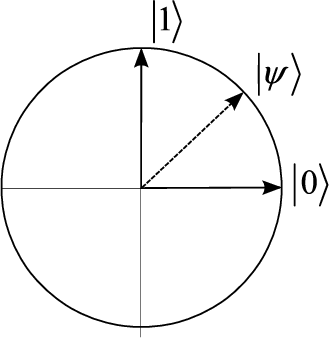
\includegraphics[scale=.3]{qubit_vector}
\end{figure}

Podemos determinar el estado de un bit clásico a la hora de examinarlo, pero en el caso del qubit, no podemos determinar el estado cuántico de un qubit en superposición, es decir, no podemos hallar el valor de $\alpha$ y $\beta$. Lo que sí podemos hacer es \textbf{medir} el qubit, determinar si colapsa en el estado $\ket{0}$ con probabilidad $|\alpha|^2$ ó en el estado $\ket{1}$ con probabilidad $|\beta|^2$. En otra palabras, el proceso de medir un qubit, nos devuelve como salida un estado clásico al que colapsa y deja de estar en superposición de varios estados de manera simultanea.

Veamos ahora otra representación geométrica del qubit que puede resultar útil. Consideramos un qubit en estado de superposición.
\begin{equation}
\ket{\psi} = c_0\ket{0} + c_1\ket{1} 
\end{equation}
con $\|c_0|^2 + |c_1|^2 = 1$. Reescribimos la expresión en coordenadas en forma exponencial de un número complejo,
\begin{equation}
\ket{\psi} = r_0 e^{i\varphi_0}\ket{0} + r_1 e^{i\varphi_1}\ket{1}
\end{equation}
Lo multiplicamos por un escalar de módulo 1, así no alteramos su estado cuántico,
\begin{equation}
e^{-i\varphi_0}\ket{\psi} = e^{-i\varphi_0}(r_0 e^{i\varphi_0}\ket{0} + r_1 e^{i\varphi_1}\ket{1}) = 
r_0\ket{0} + r_1 e^{i(\varphi_1 - \varphi_0)}\ket{1}
\end{equation}
Tomando ahora coordenadas polares $r_0 = \cos(\theta)$, $r_1 = \sin(\theta)$ y el cambio de variables $\varphi = \varphi_1 - \varphi_0$, resulta en la siguiente expresión,
\begin{equation}
\ket{\psi} = \cos(\theta)\ket{0} + e^{i\varphi}\sin(\theta)\ket{1}
\end{equation}
Considerando $\theta$ y $\varphi$ como coordenadas de un punto en una esfera tridimensional, podemos ver el estado del qubit como un punto en la superficie de dicha esfera, siendo los polos los estados $\ket{0}$ y $\ket{1}$. Esta esfera recibe el nombre de \textbf{esfera de Bloch} y veremos en poco que con ella podemos representar operaciones de qubits como rotaciones de la esfera.

\begin{figure}
	\centering
	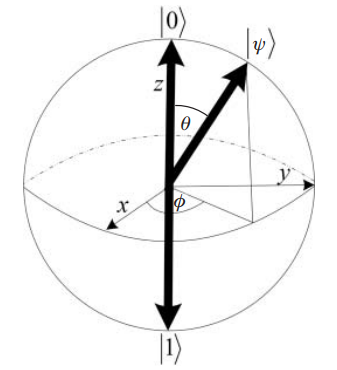
\includegraphics[scale=.3]{esfera_bloch}
	\caption{Esfera de Bloch.}
\end{figure}


\subsection{Sistema de Varios Qubits}

Tomamos interés en un sistema de un número mayor de qubits, que enlazaremos a través del producto tensorial de los espacios vectoriales. Por tanto un elemento de él estará representado por un vector de $\mathbb{C}^2 \otimes \mathbb{C}^2 \otimes \ldots \otimes \mathbb{C}^2$ que denotaremos como $(\mathbb{C}^2)^{\otimes n}$ donde $n$ es el número de qubits del sistema y cuya dimensión como espacio vectorial es $2^n$

Por ejemplo, si queremos un sistema de 2 qubits en comparación a los estados clásicos de un bit tendríamos 00, 01, 10 y 11, por tanto nuestro sistema de 2 qubits tendría los estados $\ket{00}$, $\ket{01}$, $\ket{10}$ y $\ket{11}$ que se corresponden con el producto tensorial del estado de los dos qubits $\ket{x}\otimes\ket{y}$ con $x$, $y\in \lbrace 0, 1\rbrace$.
Vamos a trabajar más cómodamente con coordenadas del vector en su expresión matricial, consideramos primero,
\begin{equation}
\ket{0} = \begin{bmatrix}
	1 \\ 0
\end{bmatrix}, \ 
\ket{1} = \begin{bmatrix}
	0 \\ 1
\end{bmatrix}
\end{equation}
Como hemos visto en la sección anterior, aplicaremos el producto de  Kroner para obtener las expresiones matriciales de $\ket{00}$, $\ket{01}$, $\ket{10}$ y $\ket{11}$,
\begin{equation}
\ket{00} =
\begin{bmatrix}
	1 \\ 0 \\ 0 \\ 0
\end{bmatrix}, \ 
\ket{01} =
\begin{bmatrix}
	0 \\ 1 \\ 0 \\ 0
\end{bmatrix}, \ 
\ket{10} =
\begin{bmatrix}
	0 \\ 0 \\ 1 \\ 0
\end{bmatrix}, \ 
\ket{11} =
\begin{bmatrix}
	0 \\ 0 \\ 0 \\ 1
\end{bmatrix}
\end{equation}
Observamos que forman una base ortonormal de un espacio vectorial de dimensión $2^2 = 4$ y que además cada coordenada corresponde a un estado clásico del qubit:
\begin{equation}
\ket{01} =
\begin{matrix}
	\textbf{00} \\ \textbf{01} \\ \textbf{10} \\ \textbf{11}
\end{matrix}
\begin{bmatrix}
	0 \\ 1 \\ 0 \\ 0
\end{bmatrix}
\end{equation}
Por tanto, si tomamos un sistema de dos qubits arbitrario en superposición,
\begin{equation}
\ket{\psi} = c_0 \ket{00} + c_1 \ket{01} + c_2 \ket{10} + c_3 \ket{11}
\end{equation}
su representación matricial sería:
\begin{equation}
\ket{\psi} =
\begin{matrix}
	\textbf{00} \\ \textbf{01} \\ \textbf{10} \\ \textbf{11}
\end{matrix}
\begin{bmatrix}
	c_0 \\ c_1 \\ c_2 \\ c_3
\end{bmatrix}
\end{equation}
Trabajaremos a partir de ahora con la notación del sistema de varios qubits como $\ket{xy}$, $\ket{x\otimes y}$, ó $\ket{x}\otimes\ket{y}$ y los trataremos de manera indiferente según convenga.


(poner estados de bell y entagled)
\subsection{Puertas Cúanticas}

La manera de trabajar y operar con los bits es a través de las puertas lógicas. Igual que hemos asociado con vectores a los bits, y podemos operar con los vectores de forma matricial, las puertas lógicas están asociados a las matrices.

Tomemos con ejemplo la puerta NOT, que funcione de la siguiente manera. NOT transformará el bit $\ket{0}$ en $\ket{1}$ y transformará el bit $\ket{1}$ en $\ket{0}$. Es decir, es la operación lógica $\neg$.

Por tanto si tomamos la matriz $\textrm{NOT} = \begin{bmatrix} 0 & 1 \\ 1 & 0 \end{bmatrix}$,
esta matriz cumple que
\begin{equation}
\begin{bmatrix}
0 & 1 \\
1 & 0
\end{bmatrix}
\begin{bmatrix}
1 \\ 0
\end{bmatrix} =
\begin{bmatrix}
0 \\ 1
\end{bmatrix}
\textrm{ y }
\begin{bmatrix}
0 & 1 \\
1 & 0
\end{bmatrix}
\begin{bmatrix}
0 \\ 1
\end{bmatrix} =
\begin{bmatrix}
1 \\ 0
\end{bmatrix}
\end{equation}

Es decir, tenemos que la puerta NOT,
\begin{equation}
\textrm{NOT} \ket{0} = \ket{1} \textrm{ y } \textrm{NOT}\ket{1} = \ket{0}
\end{equation}

Una observación es que estas matrices no tiene que ser necesariamente cuadradas. Por ejemplo, la puerta AND que queremos que tome dos bits y le aplique la operación lógica $ \wedge $.
Para ello, tomaremos la matriz $\textrm{AND} = \begin{bmatrix}
1 & 1 & 1 & 0 \\
0 & 0 & 0 & 1
\end{bmatrix}$ que satisface,
\begin{equation}
\begin{bmatrix}
1 & 1 & 1 & 0 \\
0 & 0 & 0 & 1
\end{bmatrix}
\begin{bmatrix}
0 \\ 0 \\ 0 \\ 1
\end{bmatrix} =
\begin{bmatrix}
0 \\ 1
\end{bmatrix}
\end{equation}
Es decir, $\textrm{AND}(\ket{1}\otimes\ket{1}) = \textrm{AND}\ket{11} = \ket{1}$.
Además también cumple,
\begin{equation}
\begin{bmatrix}
1 & 1 & 1 & 0 \\
0 & 0 & 0 & 1
\end{bmatrix}
\begin{bmatrix}
1 \\ 0 \\ 0 \\ 0
\end{bmatrix} =
\begin{bmatrix}
1 \\ 0
\end{bmatrix}
\textrm{, }
\begin{bmatrix}
1 & 1 & 1 & 0 \\
0 & 0 & 0 & 1
\end{bmatrix}
\begin{bmatrix}
0 \\ 1 \\ 0 \\ 0
\end{bmatrix} =
\begin{bmatrix}
1 \\ 0
\end{bmatrix}
\textrm{, y }
\begin{bmatrix}
1 & 1 & 1 & 0 \\
0 & 0 & 0 & 1
\end{bmatrix}
\begin{bmatrix}
0 \\ 0 \\ 1 \\ 0
\end{bmatrix} =
\begin{bmatrix}
1 \\ 0
\end{bmatrix}
\end{equation}
Es decir, $\textrm{AND}\ket{00} = \ket{0}$, $\textrm{AND}\ket{01} = \ket{0}$, y $\textrm{AND}\ket{10} = \ket{0}$.

De la misma manera podemos obtener por ejemplo la matriz asociada a la operación $\vee$, que llamaremos como puerta $\textrm{OR} = \begin{bmatrix}
0 & 1 & 1 & 1 \\
1 & 0 & 0 & 0
\end{bmatrix}$.

En cuanto a concatenar las puertas en un circuito, se representará por productos de matrices de manera natural. Por ejemplo si queremos aplicar primero la puerta AND seguido de la puerta NOT,
\begin{equation}
\textrm{NOT}\cdot\textrm{AND} =
\begin{bmatrix}
0 & 1 \\
1 & 0
\end{bmatrix} \cdot
\begin{bmatrix}
1 & 1 & 1 & 0 \\
0 & 0 & 0 & 1
\end{bmatrix} =
\begin{bmatrix}
0 & 0 & 0 & 1 \\
1 & 1 & 1 & 0
\end{bmatrix}
\end{equation}

También podemos realizar operaciones de manera paralela a distintos bits a través de productos tensoriales entre las matrices, siempre cuidando el tamaño de las matrices. Por ejemplo si $A$ es una puerta que recibe 2 bits como entrada y devuelve 2 bits como salida, luego $B$ es una puerta con 1 bit de entrada y 1 de salida, y queremos aplicar primero $A$ a dos bits y después la puerta $B$ al primer bit, la matriz correspondiente sería,
\begin{equation}
(B \otimes I) \cdot A
\end{equation} 
Observamos que A es una matriz 4 por 4 y $B$ es una matriz 2 por 2, por lo que no podremos realizar el producto de los dos para componer las dos aplicaciones. Para completar la matriz $B$ tomaremos la matriz identidad y le aplicaremos el producto tensorial con $B$, que interpretaremos como aplicar la matriz identidad al segundo bit.

Observamos que en los vectores que estamos usando en los ejemplos son solos $\ket{0}$ y $\ket{1}$. Ya que no tiene sentido que estas puertas tengan como entrada bits distintos de $\ket{0}$ y $\ket{1}$, no permitiremos su uso en las puertas clásicas. Veremos que a continuación, esto no será un problema para las puertas cuánticas.

Una propiedad que les pediremos a las puertas cuánticas es que sean reversibles. Esto es que dados la salida y la operación aplicada seamos capaces de determinar la entrada del circuito. Representaremos las puertas cuánticas con matrices unitarias que son reversibles por su propia adjunta. Recordemos que esto es:
\begin{equation}
U * U^\dagger = U^\dagger * U = I_n
\end{equation}

Por ejemplo una puerta que cumple esta propiedad es la puerta NOT controlada.
(Poner puerta en un circuito)
Esta puerta tomará dos entradas y dará dos salidas. La primera entrada la llamaremos bit de control, es decir, controlará el bit de salida. Si $\ket{x} = \ket{0}$, la salida del segundo bit $\ket{y}$ permanecerá igual. Si  $\ket{x} = \ket{1}$ entonces $\ket{y}$ se le aplicará la puerta NOT, es decir, será lo contrario.
Esto se puede ver como que la puerta transforma un par de bits $\ket{x, y}$ en $\ket{x, x\oplus y}$, donde $\oplus$ es la operación binaria de OR excluyente, o también como la suma en módulo 2.

La matriz correspondiente a esta puerta sería:
\begin{equation}
\textrm{CNOT} = \begin{bmatrix}
1 & 0 & 0 & 0 \\
0 & 1 & 0 & 0 \\
0 & 0 & 0 & 1 \\
0 & 0 & 1 & 0 
\end{bmatrix}
\end{equation}
Observamos que claramente esta puerta es unitaria pues el producto por su adjunta que es ella misma resulta en la matriz identidad:
\begin{equation}
\begin{bmatrix}
1 & 0 & 0 & 0 \\
0 & 1 & 0 & 0 \\
0 & 0 & 0 & 1 \\
0 & 0 & 1 & 0 
\end{bmatrix}
\begin{bmatrix}
1 & 0 & 0 & 0 \\
0 & 1 & 0 & 0 \\
0 & 0 & 0 & 1 \\
0 & 0 & 1 & 0 
\end{bmatrix} = 
\begin{bmatrix}
1 & 0 & 0 & 0 \\
0 & 1 & 0 & 0 \\
0 & 0 & 1 & 0 \\
0 & 0 & 0 & 1 
\end{bmatrix}
\end{equation}
Esto también se puede entender como que la puerta CNOT es reversible por ella misma:
(Poner circuito)
El estado de entrada es $\ket{x, y}$ que queda trasformado en $\ket{x, x\oplus y}$ y esta última en $\ket{x, x\oplus (x\oplus y)}$. Esto es $\ket{x, (x\oplus x) \oplus y} = \ket{x, 0\oplus y} = \ket{x, y}$, ya que $x\oplus x = 0$.

Otra puerta reversible de mucha importancia es es la de Toffoli,
que funciona de manera similar a la puerta NOT controlada. Trabaja con 3 bits de entrada y salida, en el que aplica la puerta NOT al último bit $\ket{z}$ si y solo si los dos anteriores tienen por estado 1, $\ket{x, y} = \ket{11}$. En otras palabras lleva el $\ket{x,y,z}$ a $\ket{x,y,z\oplus(x\wedge y)}$.
Esta puerta tiene por matriz:
\begin{equation}
\begin{bmatrix}
1 & 0 & 0 & 0 & 0 & 0 & 0 & 0 \\
0 & 1 & 0 & 0 & 0 & 0 & 0 & 0 \\
0 & 0 & 1 & 0 & 0 & 0 & 0 & 0 \\
0 & 0 & 0 & 1 & 0 & 0 & 0 & 0 \\
0 & 0 & 0 & 0 & 1 & 0 & 0 & 0 \\
0 & 0 & 0 & 0 & 0 & 1 & 0 & 0 \\
0 & 0 & 0 & 0 & 0 & 0 & 0 & 1 \\
0 & 0 & 0 & 0 & 0 & 0 & 1 & 0
\end{bmatrix}
\end{equation}

Ya hemos visto varias puertas que son reversibles, ahora, llamaremos puertas cuánticas a aquellas aplicaciones que actúan sobre qubits, como vectores de un espacio vectorial complejo y tendrá como representación matricial, matrices unitarias.

Otra puerta cuántica de mucha importancia es la puerta de Hadamard ya que nos permitirá poner qubit en superposición, es decir, en una configuración en la que todos los estados son equiprobables. Esta puerta tiene por matriz:
\begin{equation}
\frac{1}{\sqrt{2}}
\begin{bmatrix}
1 & 1 \\
1 & -1
\end{bmatrix}
\end{equation}

Una excepción de las puertas cuánticas sería la operación de medir un qubit, que se suelen realizar al final del circuito y que no son reversibles.




\begin{comment}
Organización
-Otro ejemplo con OR y AND.
-Solo operable con ket0 y ket1, luego relacionar con puertas cuánticas.
-Se puede concatenar operaciones que es producto de matrices.
-También de manera paralela con bits diferentes. Poner ejemplo.
-Importancia en puertas reversibles (Preguntar).
-Puertas Cuánticas, poner ejemplos y hablar de los dibujos de los circuitos.
-Hablar del qubit representado en la esfera de Bosch.
\end{comment}


\newpage

\section{Algoritmos Cuánticos}

En general, los algoritmos cuánticos siguen un esquema común entre ellos. Estos consistirán en:
\begin{itemize}
\item Comenzaremos con una serie de qubits en su estado clásico, es decir, $\ket{0}$ ó $\ket{1}$
\item Luego, serán puestos en superposición de varios estados.
\item Se le aplicarán una serie de operaciones unitarias a través de puertas cuánticas.
\item Y finalmente se medirán los qubits correspondientes y según el algoritmo, se repetirá este proceso varias veces y se compararán los resultados.

\end{itemize}

\subsection{Algoritmo de Deutsch}

El primer algoritmo que veremos y el más simple será el algorimto de Deutsch. Este algoritmo tratará de ver si se cumple cierta propiedad para una función $f:\{0, 1\} \rightarrow \{0, 1\}$, concretamente si es balanceada o constante.

\begin{deff}
Diremos que la función $f:\{0, 1\} \rightarrow \{0, 1\}$ es balanceada si $f(0) \neq f(1)$, y diremos que es constante si $f(0) = f(1)$.
\end{deff}

El algoritmo consistirá en tomar una función $f:\{0, 1\} \rightarrow \{0, 1\}$, con la sólo podemos evaluar la función y obtener la imagen y no sabemos cómo está definido la función y determinar si la función es balanceada o constante.

Para ello tomaremos una puerta cuántica que evaluará la función y observamos que esta tiene que ser reversible. Consideraremos la siguiente operación unitaria $U_f$. A esta función a veces nos referiremos como oráculo, ya que nos evaluará la función indicando la imagen sin que nosotros sepamos la definición de la función.

(Poner circuito)

En la primera entrada $\ket{x}$ será lo que queremos evaluar, y en la segunda entrada $\ket{y}$ actuará como un qubit de control. Tras el cuál, en la primera salida $\ket{x}$ permanecerá igual y en la segunda salida tendremos $\ket{y\oplus f(x)}$.

Observamos que esta puerta cuántica es reversible pues:

(Poner circuito)

El estado $\ket{x, y}$ queda trasformado en $\ket{x, y\oplus f(x)}$ y posteriormente en $\ket{x, (y\oplus f(x))\oplus f(x)} = \ket{x, y\oplus (f(x)\oplus f(x))} = \ket{x, y\oplus 0} = \ket{x, y}$.

El circuito del algoritmo consistirá en lo siguiente:

(Poner circuito)

Esto en términos matriciales sería:
\begin{equation}
(H\oplus I) U_f (H\oplus H) \ket{0, 1} = 
(H\oplus I) U_f (H\oplus H)
\begin{bmatrix}
0 \\ 1 \\ 0 \\ 0
\end{bmatrix}
\end{equation}
Veamos en detalle el resultado al que se llega. Empezamos con el estado $\ket{\varphi_0} = \ket{0, 1}$ que pondremos en superposición con la puerta de Hadamard.
Hadamard transforma a $\ket{0}$ en $\frac{\ket{0} + \ket{1}}{\sqrt{2}}$ y $\ket{1}$ en $\frac{\ket{0} - \ket{1}}{\sqrt{2}}$, por tanto,
\begin{equation}
\ket{\varphi_1} = \left[ \frac{\ket{0} + \ket{1}}{\sqrt{2}} \right] \left[ \frac{\ket{0} - \ket{1}}{\sqrt{2}} \right] =
\frac{\ket{0,0} - \ket{0,1} + \ket{1,0} - \ket{1,1}}{2} = 
\begin{bmatrix}
+\frac{1}{2} \\ -\frac{1}{2} \\ +\frac{1}{2} \\ -\frac{1}{2}
\end{bmatrix}
\end{equation}
Ahora, aplicaremos el oráculo $U_f$ a la expresión $\frac{\ket{0,0} - \ket{0,1} + \ket{1,0} - \ket{1,1}}{2}$ y recordando que $U_f$ no deja de ser una aplicación lineal. Por tanto, tenemos que
\begin{equation}
\ket{\varphi_2} = U_f \frac{\ket{0,0} - \ket{0,1} + \ket{1,0} - \ket{1,1}}{2} = \frac{U_f\ket{0,0} - U_f\ket{0,1} + U_f\ket{1,0} - U_f\ket{1,1}}{2} 
\end{equation}
Recordemos que nuestro oráculo $U_f$ transforma $\ket{x,y}$ en $\ket{x,y\oplus f(x)}$, por lo que
\begin{equation}
\begin{split}
\ket{\varphi_2} =
\frac{\ket{0,0\oplus f(0)} - \ket{0,1\oplus f(0)} + \ket{1, 0\oplus f(1)} - \ket{1, 1\oplus f(1)}}{2} = \\
\frac{\ket{0,f(0)} - \ket{0,\overline{f(0)}} + \ket{1,f(1)} - \ket{1,\overline{f(1)}}}{2}
\end{split}
\end{equation}
donde $\overline{f(x)}$ es el contrario de $f(x)$.

Recordemos que $\ket{x,y}$ no es más que una notación de $\ket{x}\otimes\ket{y}$, por tanto aplicando la propiedad distributiva del producto tensorial por la derecha tenemos
\begin{equation} \label{eq45}
\ket{\varphi_2} =
\frac{\ket{0} \otimes \left[ \ket{f(0)} - \ket{\overline{f(0)}} \right] + \ket{1} \otimes \left[ \ket{f(1)} - \ket{\overline{f(1)}} \right]}{2}
\end{equation}
Observemos en un momento la expresión $\ket{f(x)} -\ket{\overline{f(x)}}$ para $x \in \lbrace 0,1 \rbrace$ y discutimos su valor según el valor de $f(x)$.
\begin{equation}
\ket{f(x)} - \ket{\overline{f(x)}} =
\begin{Bmatrix}
\ket{0} - \ket{1} & \textrm{si} & f(x) = 0 \\
\ket{1} - \ket{0} & \textrm{si} & f(x) = 1
\end{Bmatrix}
\end{equation}
que escribiremos como $(-1)^{f(x)}(\ket{0} - \ket{1})$.

Aplicando esto a la expresión \ref{eq45} tenemos que
\begin{equation}
\ket{\varphi_2} = 
\frac{(-1)^{f(0)} (\ket{0} \otimes \left[ \ket{0} - \ket{1} \right]) + (-1)^{f(1)} (\ket{1} \otimes \left[ \ket{0} - \ket{1} \right])}{2}
\end{equation}
Hacemos uso de la propiedad distributiva por la derecha y reordenamos los escalares para separar la expresión en producto escalar de dos términos
\begin{equation}
\ket{\varphi_2} =
\left[ \frac{(-1)^{f(0)} \ket{0} + (-1)^{f(1)} \ket{1}}{\sqrt{2}} \right]
\left[ \frac{\ket{0} - \ket{1}}{\sqrt{2}} \right]
\end{equation}
Discutamos el valor de la expresión $(-1)^{f(0)} \ket{0} + (-1)^{f(1)} \ket{1}$ según si $f(x)$ es constante o balanceada.
\begin{equation}
\ket{\varphi_2} = 
\begin{cases}
(\pm 1) \left[\frac{\ket{0}+\ket{1}}{2}\right] \left[\frac{\ket{0}-\ket{1}}{2}\right] & \textrm{si } f \textrm{ es constante,} \\
(\pm 1) \left[\frac{\ket{0}-\ket{1}}{2}\right] \left[\frac{\ket{0}-\ket{1}}{2}\right] & \textrm{si } f \textrm{ es balanceada.}
\end{cases}
\end{equation}
Teniendo en cuenta que Hadamard es su propia inversa, llevará $\frac{\ket{0}+\ket{1}}{2}$ a $\ket{0}$ y $\frac{\ket{0}-\ket{1}}{2}$ a $\ket{1}$.
\begin{equation}
\ket{\varphi_3} = 
\begin{cases}
(\pm 1) \ket{0} \left[\frac{\ket{0}-\ket{1}}{2}\right] & \textrm{si } f \textrm{ es constante,} \\
(\pm 1) \ket{1} \left[\frac{\ket{0}-\ket{1}}{2}\right] & \textrm{si } f \textrm{ es balanceada.}
\end{cases}
\end{equation}
Finalmente medimos el qubit superior para determinar si f es constante o balanceada, ya que si sale $\ket{0}$ será constante y si sale $\ket{1}$ será balanceada. Observamos que el signo no afecta a la proceso de medir, pues recordemos que la probabilidad de que sea un estado depende de la norma al cuadrado.

\scalebox{2.0}{
\Qcircuit @C=1.0em @R=0.2em @!R { \\
	 	\nghost{{q}_{0} :  } & \lstick{{q}_{0} :  } & \gate{\mathrm{H}} & \qw & \qw & \qw\\
	 	\nghost{{q}_{1} :  } & \lstick{{q}_{1} :  } & \gate{\mathrm{H}} & \ctrl{1} & \qw & \qw\\
	 	\nghost{{q}_{2} :  } & \lstick{{q}_{2} :  } & \qw & \targ & \qw & \qw\\
	 	\nghost{\mathrm{{c} :  }} & \lstick{\mathrm{{c} :  }} & \lstick{/_{_{1}}} \cw & \cw & \cw & \cw\\
\\ }}




\newpage

%Espacios de Hilbert Referencias

%Corregir llaves(HECHO)

%En qubits porner la representación de la esfera de Bloch(HECHO)

%Poner ejemplos de qubts multiples

%Poner ejemplos de circuitos

%PONER MÁS PROPIEDADES DEL PRODUCTO TENSORIAL COMO OPERADOR(HECHO)

%Puerta de teleportación ejemplo en algoritmos cuánticos

%En algoritmo de Deutsch indicar la eficiencia

%Traducir entagled

\section{Conclusión}

%e must clarify what we mean by “simulate.” In the classical world, we say that one circuit Circ simulates another circuit Circ	 if for any possible inputs, the output for Circ will be the same for Circ	

%Things in the quantum world are a tad more complicated. Because of the probabilistic nature of quantum computation, the outputs of a circuit are always probabilistic. So we have to reformulate what we mean when we talk about simulate. We shall not worry about this here.

\newpage

\section{Bibliografía}
%Dos libros...

%https://es.wikipedia.org/wiki/Espacio_vectorial

%https://en.wikipedia.org/wiki/Tensor_product

%https://ctan.org/pkg/braket



\end{document}